\documentclass[12pt]{article}
\usepackage{ucs}
\usepackage[utf8x]{inputenc}
\usepackage[turkish,english]{babel}
\usepackage{graphicx}
\usepackage{url}
\usepackage[sc]{mathpazo}
\linespread{1.05}
\usepackage[T1]{fontenc}
\usepackage[a2paper,margin=1cm]{geometry}
\usepackage{shapepar}
\pagestyle{empty}

\author{Mehmet Atakan Gürkan}
\title{}
\date{}
\newcommand\almleftshape{
   {0}
   {0}b{0}
\\ {0}t{0}{7}
\\ {12}t{0}{9.5}
\\ {19}t{0}{9.7}
\\ {21}t{0}{9.7}
\\ {24}t{0}{9.3}
\\ {34}t{0}{6.3}
\\ {40}t{0}{4.6}
\\ {41}e{0}}
\newcommand\almrightshape{
   {12}
   {0}b{0}
\\ {0}t{3.2}{6.8}
\\ {1}t{4}{6}
\\ {5}t{2.6}{7.4}
\\ {10}t{1.0}{9}
\\ {15}t{-0.6}{10.6}
\\ {17}t{-1}{11.0}
\\ {19}t{-1.2}{11.2}
\\ {21}t{-1}{11.0}
\\ {27}t{0}{10.0}
\\ {41}t{3.5}{6.5}
\\ {42}e{10}}
\begin{document}
%\maketitle
\shorthandoff{=}
\centerline{\raisebox{-24pt}{\includegraphics[clip,height=72pt]{logolar/ODTU_KKK_logo.pdf}}
     \fontsize{40pt}{40pt}\selectfont
     \,\,için Gökyüzü Almanağı / Sky Almanac for\,
\raisebox{-24pt}{\includegraphics[clip,height=72pt]{logolar/METU_NCC_logo.pdf}}}
\noindent\centerline{\fontsize{36pt}{36pt}\selectfont2015}
\vskip 1cm
\noindent
\centerline{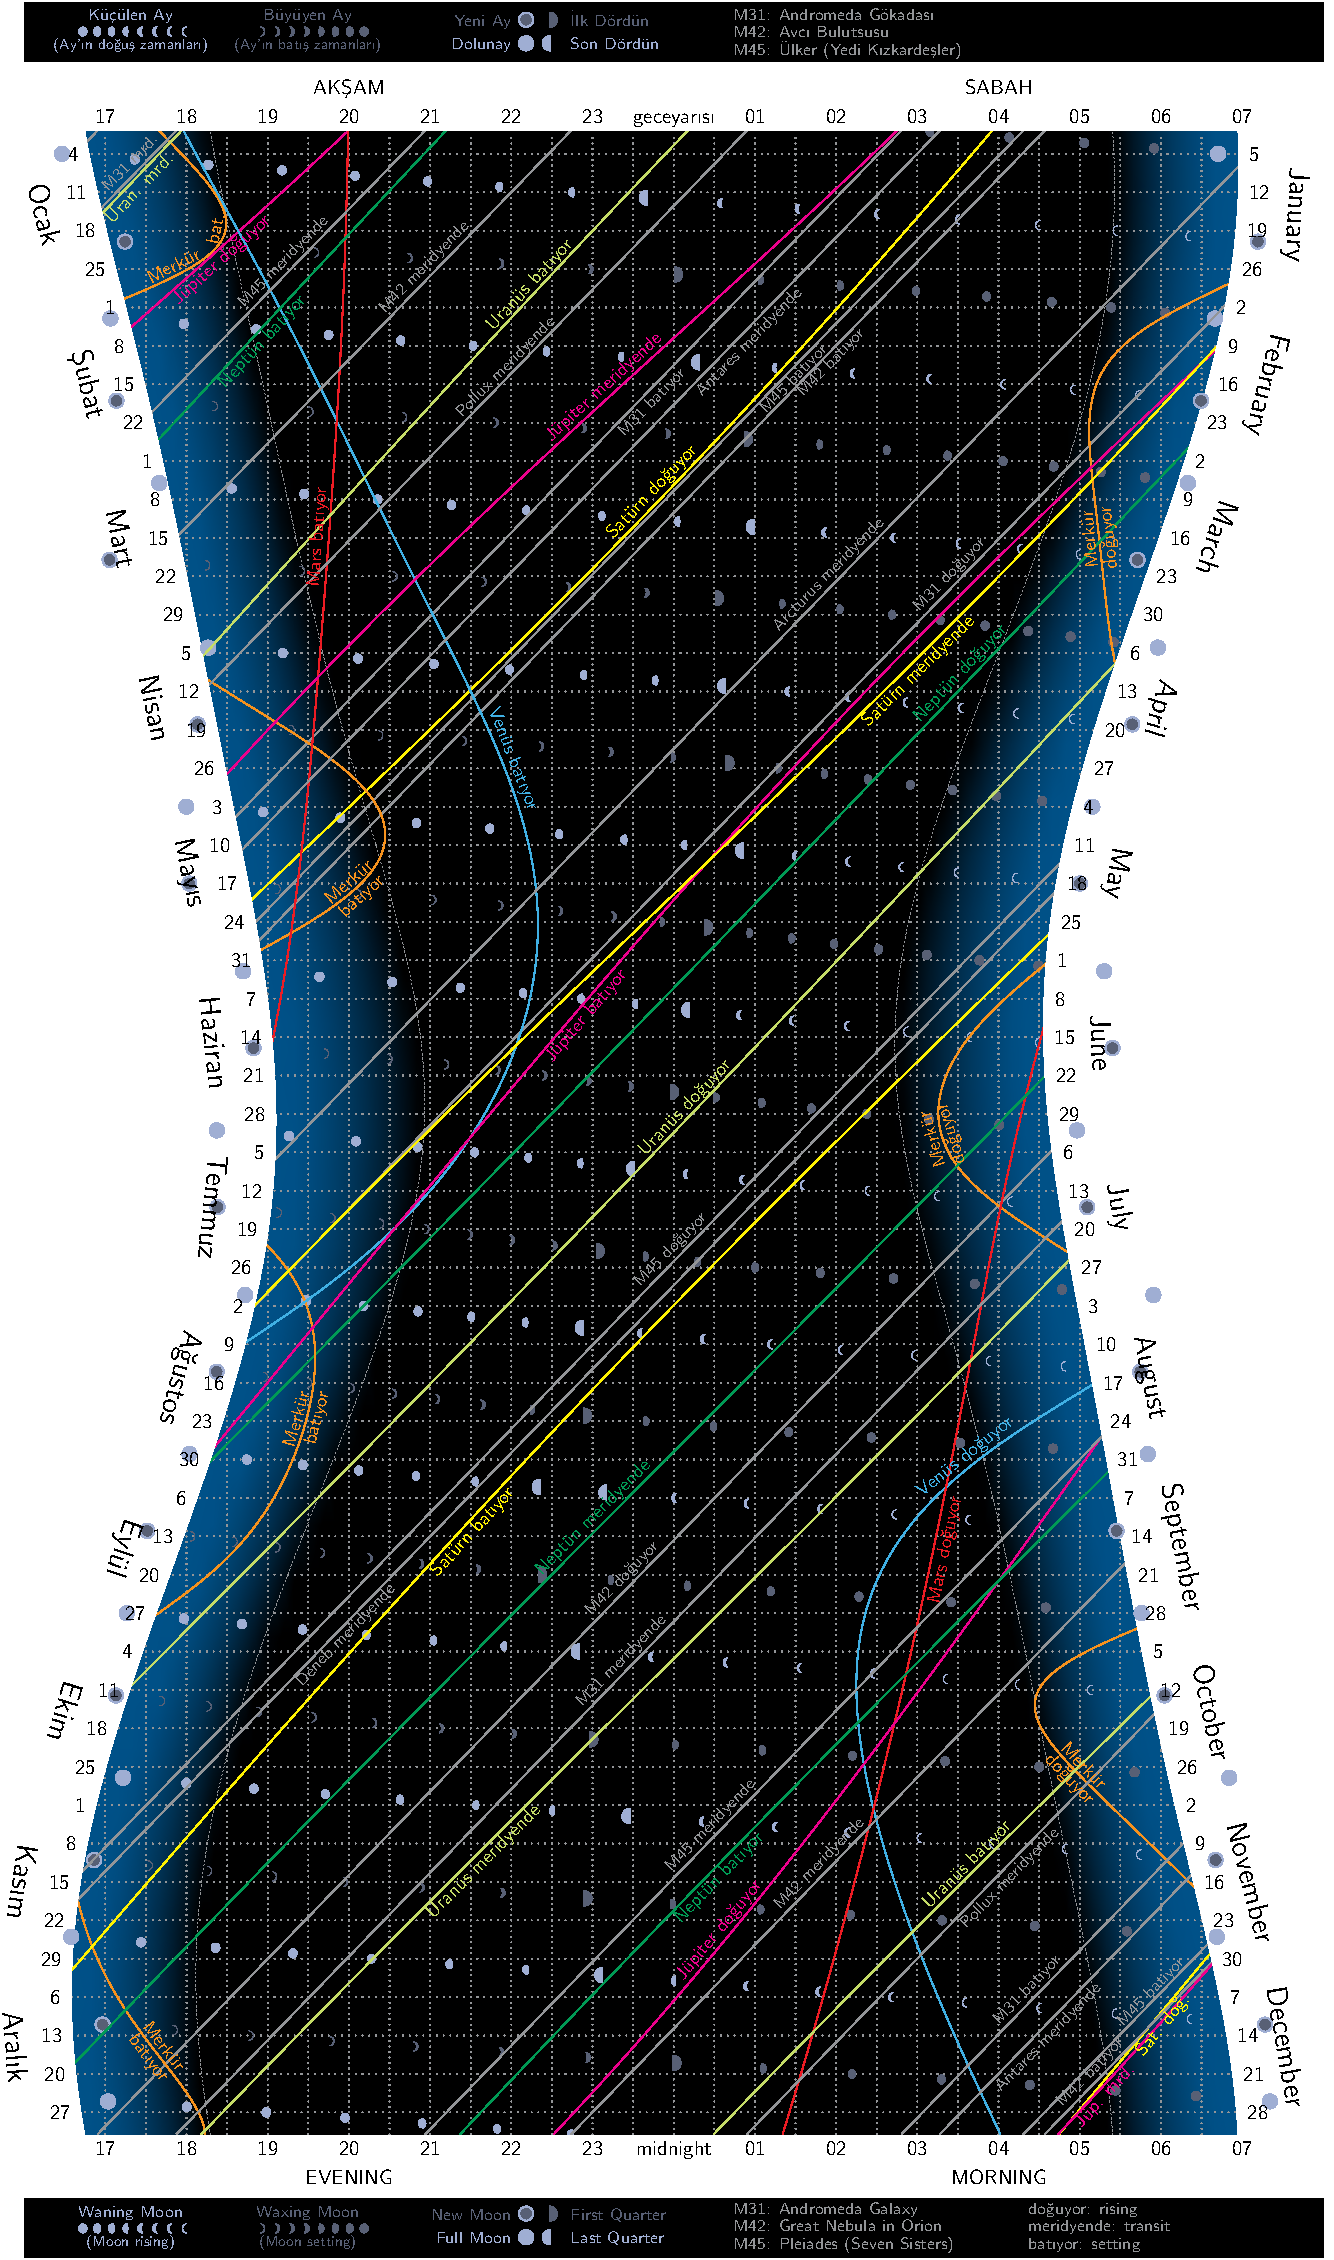
\includegraphics[clip,height=0.9\textheight]{almanac_2015_ODTUKKK}}

\vskip -0.9\textheight \vskip9cm
\noindent
\cutout{l}(0cm,0pt)
\shapepar{\almleftshape}{\fontsize{13pt}{13pt}\selectfont
\selectlanguage{turkish}
\hskip0.4cm\textbf{Çizelgenin Kullanımı}\\
Bu çizelge, 2015 yılı için, ODTÜ Kuzey Kıbrıs Kampüsü'nde çeşitli
gök cisimlerinin doğma, meridyenden (gökyüzünde ulaştıkları en
yüksek noktadan) geçme ve batma zamanlarını, alacakaranlığın
sonuyla başlangıcını ve Ay'ın evrelerini veriyor.  Dikey eksen
günleri, yatay eksen gece boyunca zamanı gösteriyor.  Gece içinde
yarımşar saatlik aralıklar ve yıl içinde Pazar akşamlarını
Pazartesi sabahlarına bağlayan geceler noktalı çizgilerle
belirtiliyor. Düşey olarak iki nokta arası bir güne, yatay olarak
iki nokta arası beş dakikaya karşılık geliyor.\\
Bir örnek olarak 9 Mart gecesinin olaylarına bakarsak: İlk olarak,
sol tarafta 8 Mart'a karşılık gelen noktanın hemen altında, yaklaşık
olarak 9 Mart'a karşılık gelen noktayı bulmak gerekiyor. Bu noktaya
yukarıda karşılık gelen zaman (17:50) Güneş'in batma zamanı. Buradan
sağa doğru ilerlediğimizde 18:15 civarında M42'nin (Avcı Bulutsusu)
meridyenden geçtiğini yani gökyüzünde ulaşacağı en yüksek
noktada olacağını görüyoruz. Yaklaşık 19:45'de Mars batıyor.
Buradan, Güneş battığı zaman
Mars'ın gökyüzünde olduğunu da çıkarabiliriz. Mars'ın hemen ardından
Uranüs 19:50'de batıyor (Uranüs'ü çıplak gözle göremeyiz). Bunu 20:20'de
Venüs'ün batışı, 20:25'te
Pollux'un meridyenden geçişi ve 21:17'de Ay'ın doğuşu izliyor. Bugün
doğan Ay dolunay ile son dördün arasında bir büyüklükte. Bu biçimde
devam ettikçe Jüpiter'in meridyenden geçişinin, M31'in batışının,
Antares'in meridyenden geçişinin ve diğer bazı gök olaylarının zamanlarını
da bulabiliriz. 19:16 ve 4:40 civarında
gördüğümüz kesikli çizgiler sırasıyla alacakaranlığın
bitmesi ve başlamasını belirtiyor. Bu noktalar Güneş'in ufkun
18$^\circ$ altında kaldığı anlara karşılık geliyor.\\
Çizelgede verilen doğma ve batma zamanları, ufuk çizgisinin önünde bir engel
olmadığını varsayıyor. Eğer böyle bir engel varsa, her bir
açı derecesi yükseklik için doğma zamanı 4 dakika geç, batma zamanı da
aynı miktarda erken olacak. Benzer biçimde, yüksek bir nokta\-dan gözlem
yapıldığı için ufuk çizgisi olması gerekenin altında ise, doğma ve batma
zamanlarının düzeltilmesi gerekecek.\\
Not: Yaz saati uygulamasının olduğu zamanlarda,
çizelgedeki zamanlara
bir~saat eklemek gerekiyor.\\~\\~
}
\vskip -6.7cm
\cutout{r}(2em,6cm)
\shapepar{\almrightshape}{\fontsize{13pt}{13pt}\selectfont
\selectlanguage{english}
\hskip 1.2cm\textbf{Using the Chart}\\
This chart gives the rise, transit (reaching the highest point in
the sky) and setting time for various stellar objects, the end and the
beginning of the twilight, and the phases of the Moon for METU Northern
Cyprus Campus in the year 2015. The vertical axis denotes the days and
the horizontal axis denotes the time through the night. Every half
hour during the night and the nights connecting Sunday evenings to Monday
mornings are indicated by dotted lines. Each point corresponds to a day
for the vertical lines and to five minutes for the horizontal lines.\\
As an example, let's look at the night of March 9$^\textrm{th}$:
First of all, we need to find the point corresponding to March 9, just
below March 8 mark on the left. The time corresponding to this point
at the top (17:50) is
the time for sunset. As we proceed towards right from this point,
we see that M42 (The Orion Nebula) transits around 18:15.
This is followed by Mars setting at about 19:45, from which we can
deduce that it was on the sky when the Sun set. Right after Mars, Uranus
sets at about 19:50 (Uranus is not visible to the naked eye). This is
followed by Venus setting at 20:20, Pollux's transit at 20:25 and the Moon rising at 21:17. This
rising Moon is smaller than full moon but larger than last quarter. As
we continue this way, we figure out the times for Jupiter's transit,
M31's setting, Antares's transit etc. through the night. The dashed lines
around 19:16 and 4:40 indicate the end of the evening
twilight and the beginning of the morning twilight. These points are
determined by calculating the time that Sun is 18$^\circ$ below
horizon.\\
The rise and set times in the chart are calculated by assuming that
there is no obstacle in front of the horizon. If there is such an
obstacle, for each degree angle of its height rising time will be 4
minutes late and setting time 4 minutes early. Likewise, if the horizon
is below horizontal level, an opposite adjustment has to be made.\\
PS: While daylight savings time (a.k.a. summer time) is in effect,
you need to add one hour to the times given in the chart.\\ ~}
\vskip 48.5cm \footnotesize

{\hfill M. Atakan Gürkan \url{<mgurkan@metu.edu.tr>}}

{\hfill \url{https://github.com/atakan/PySkyAlmanac/2015/ODTU_KKK}}
\end{document}
